\documentclass[tikz,border=5mm]{standalone}
\usetikzlibrary{positioning}

\begin{document}
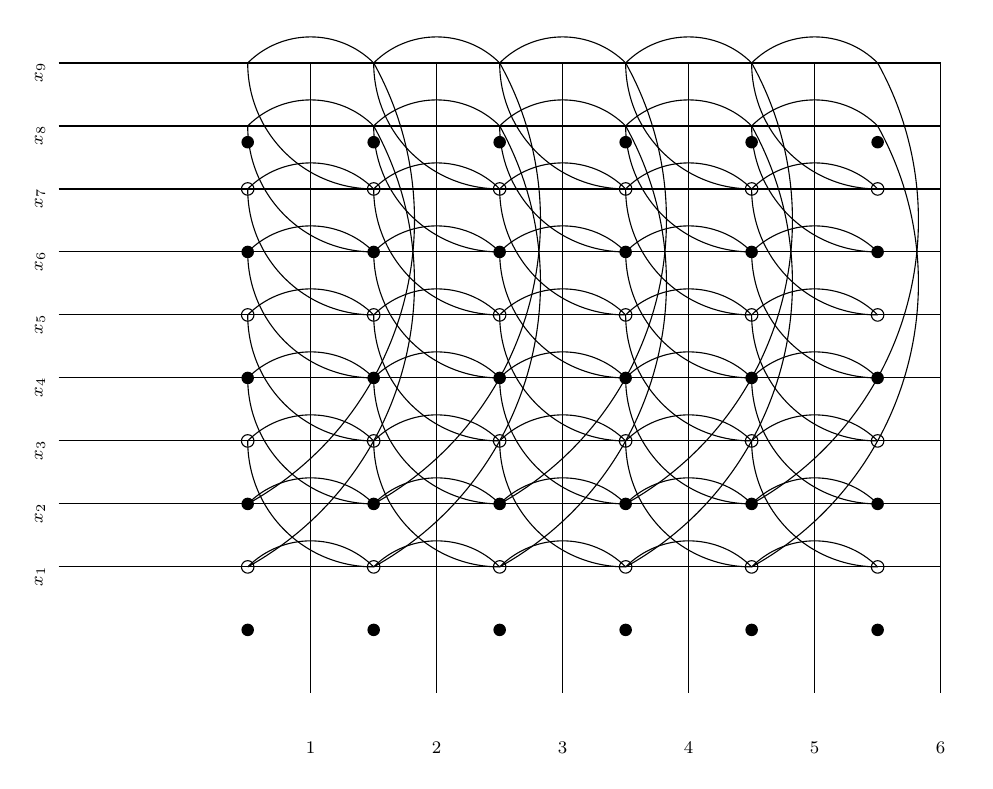
\begin{tikzpicture}[scale=0.8, transform shape]

% Define node styles
\tikzset{
    dot/.style={circle, fill, inner sep=2pt},
    circ/.style={circle, draw, inner sep=2pt},
    label/.style={below=1ex, font=\footnotesize},
}

% Draw vertical lines for x-axis
\foreach \x in {1,...,6} {
    \draw (2*\x, -2) -- (2*\x, 8);
    \node at (2*\x, -2.5) [label] {\x};
}

% Draw horizontal lines for y-axis
\foreach \y in {1,...,9} {
    \draw (-2, \y-1) -- (12, \y-1);
    \node at (-2.5, \y-1) [label, rotate=90] {$x_{\y}$};
}

% Place nodes in K_n graphs
\foreach \i in {1,...,6} {
    \node at (2*\i-1, 7) [dot, label=above:$\mathbf{\i K_9}$] {};
    \node at (2*\i-1, 6) [circ] {};
    \node at (2*\i-1, 5) [dot] {};
    \node at (2*\i-1, 4) [circ] {};
    \node at (2*\i-1, 3) [dot] {};
    \node at (2*\i-1, 2) [circ] {};
    \node at (2*\i-1, 1) [dot] {};
    \node at (2*\i-1, 0) [circ] {};
    \node at (2*\i-1, -1) [dot] {};
}

% Draw edges between nodes
\foreach \i in {1,...,5} {
    \foreach \j in {1,...,9} {
        \pgfmathtruncatemacro{\next}{mod(\j+1,9)+1}
        \draw (2*\i-1, 9-\j) to[bend left=45] (2*\i+1, 9-\j);
        \draw (2*\i-1, 9-\j) to[bend right=45] (2*\i+1, 9-\next);
    }
}

\end{tikzpicture}
\end{document}